\section{Data space estimators}

The model error in the space of data can be defined as the expectation of the
likelihood function across replicas
\begin{equation}
    \label{eq:chi2kerep}
    \erep{\repchis} = \frac{1}{\ndata} 
    \erep{ {\vecdiffreptwo}^{T} \invcov{} \vecdiffreptwo}.
\end{equation}
The data upon which this is evaluated can either be the fitted data, which 

% We start with the expectation of $\repchis$ across replicas
% \begin{equation}
%     \label{eq:chi2kerep}
%     \erep{\repchis} = \frac{1}{\ndata} 
%     \erep{ {\vecdiffreptwo}^{T} \invcov{} \vecdiffreptwo}.
% \end{equation}
It is useful perform a decomposition of this expression, as in \cite{mlforphysics}.
The differences between the cost function in the reference and that in
\eqref{eq:chi2kerep} are that our pseudodata has an additional shift, $\shift$,
and that the $\repchis$ takes into account the correlations between data points.
The decomposition can be easily performed by rotating into the basis which
diagonalises the experimental covmat. Since the covariance matrix is positive
definite, we can project $\vecdiffreptwo$ onto the eigenvectors of $\cov$
\begin{equation}
    \erep{\repchis} = \frac{1}{\ndata} \sum_{i=1}^{\ndata} \frac{(\diag{\model}^{\repind} - \diag{\levtwo}^{\repind})_i^2}{\coveig_i}
\end{equation}
where $\coveig_i$ is the eigenvalue associated with the $i^{th}$ eigenvector of
the covmat. Then we complete the square
\begin{equation}\label{eq:chi2decomp1}
    \begin{split}
        \erep{\repchis} &=
        \erep{\frac{1}{\ndata} \sum_{i=1}^{\ndata}
            \frac{
                (\diag{\model}^{\repind} - \diag{\law} + \diag{\law} - \diag{\levtwo}^{\repind})_i^2
            }{\coveig_i} } \\
        &= \erep{\frac{1}{\ndata} \sum_{i=1}^{\ndata}
            \frac{(\diag{\model}^{\repind} - \diag{\law})^2_i}{\coveig_i} +
            \frac{(\diag{\law} - \diag{\levtwo}^{\repind})_i^2}{\coveig_i} +
            \frac{2(\diag{\model}^{\repind} - \diag{\law})_i(\diag{\law} - \diag{\levtwo}^{\repind})_i}{\coveig_i}}.
    \end{split}
\end{equation}
The first term in the second line can be simplified further by completing the
square again
\begin{equation}
    \begin{split}
        \frac{1}{\ndata}\erep{\frac{(\diag{\model}^{\repind} - \diag{\law})^2_i}{\coveig_i}} &=
        \frac{1}{\ndata}\erep{\frac{(\diag{\model}^{\repind} - \erep{\diag{\model}} + \erep{\diag{\model}} - \diag{\law})^2_i}{\coveig_i}} \\
        &= \frac{1}{\ndata}\erep{\frac{(\diag{\model}^{\repind} - \erep{\diag{\model}})_i^2}{\coveig_i} +
        \frac{(\erep{\diag{\model}} - \diag{\law})^2_i}{\coveig_i} +
        \frac{2(\diag{\model}^{\repind} - \erep{\diag{\model}})_i(\erep{\diag{\model}} - \diag{\law})_i}{\coveig_i}} \\
        &= \frac{1}{\ndata}\erep{\frac{(\diag{\model}^{\repind} - \erep{\diag{\model}})_i^2}{\coveig_i}} +
        \frac{1}{\ndata}\frac{(\erep{\diag{\model}} - \diag{\law})^2_i}{\coveig_i} \\
        &= \var + \bias,
    \end{split}
\end{equation}
where we made use of the fact that $\diag{\law}$ and $\erep{\diag{\model}}$
are constant across replicas. The second term in the last line of equation
\eqref{eq:chi2decomp1} can also be slightly simplified as
\begin{equation}
    \begin{split}
        \frac{1}{\ndata}\erep{\frac{(\diag{\law} - \diag{\levtwo}^{\repind})_i^2}{\coveig_i}} &=
        \frac{1}{\ndata}\erep{\frac{(-\shift - \noise)_i^2}{\coveig_i}} \\
        &= \frac{1}{\ndata}\erep{\frac{\shift^2 + \noise^2 + 2\shift\noise)_i}{\coveig_i}} \\
        &= \frac{1}{\ndata} \left(\frac{\shift_i^2}{\coveig_i} + \frac{\erep{\noise_i^2}}{\coveig_i} \right) \\
        &= {\rm shift} + {\rm noise}
    \end{split}
\end{equation}
Finally we have the cross term,
\begin{equation}
    \begin{split}
        \frac{1}{\ndata}\frac{2(\diag{\model}^{\repind} - \diag{\law})_i(\diag{\law} - \diag{\levtwo}^{\repind})_i}{\coveig_i} &=
             - \frac{1}{\ndata} \left( \frac{2(\erep{\diag{\model}} - \diag{\law})_i\shift_i}{\coveig_i} +
             \frac{2\erep{\diag{\model_i}^{\repind} \noise_i}}{\coveig_i} \right) \\
         &= - \left( \shiftcross + \noisecross \right).
    \end{split}
\end{equation}
At this stage it's interesting to note that if the data we are calculating this
expression on is data which was not used in the fit, then the noise cross term
will go to zero, since $\diag{\model_i}^{\repind}$ and $\noise$ would be
independent. In NNPDF3.0 there was an estimator which aimed to measure
"over-fitting", $\Delta_{\chi^2}$, which using the notation here is defined as
\begin{equation}\label{eq:deltachi2def1}
    \Delta_{\chi^2} = \frac{1}{\ndata}\frac{(\erep{\diag{\model}} - \diag{\levone})_i^2 - \diag{\shift}_i^2}{\coveig_i},
\end{equation}
where we have normalised by $\ndata$ rather than in \cite{nnpdf30} which instead normalised
by $\sum_i^{\ndata} \frac{\diag{\shift}_i^2}{\coveig_i}$. It's clear that in the large
$\ndata$ limit that you would expect the two normalisations to be converge. The
idea of $\Delta_{\chi^2}$ is that it measures whether the central predictions
fit the level one data better than the underlying law. If $\Delta_{\chi^2}$
is negative then the central predictions overfit the level one data, whereas
if $\Delta_{\chi^2}$ is positive the central predictions underfit the level one
data. Ideally we would want to have $\Delta_{\chi^2}$ as close to zero as possible.
We can use the same trick of completing the square
\begin{equation}\label{eq:deltachi2def}
    \begin{split}
        \Delta_{\chi^2} &= \frac{1}{\ndata}\frac{(\erep{\diag{\model}} - \diag{\law} + \diag{\law} - \diag{\levone})_i^2 - \diag{\shift}_i^2}{\coveig_i} \\
        &= \frac{1}{\ndata}\frac{(\erep{\diag{\model}} - \diag{\law})_i^2 + (\diag{\law} - \diag{\levone})_i^2 + 2(\erep{\diag{\model}} - \diag{\law})_i(\diag{\law} - \diag{\levone})_i - \diag{\shift}_i^2}{\coveig_i} \\
        &= \bias - \shiftcross,
    \end{split}
\end{equation}
where in the second line the second and last terms cancel. The last line indicates
that $\Delta_{\chi^2}$ will likely appear in the decomposition of $\repchis$.
The first line of \eqref{eq:deltachi2def1} can be written as
\begin{equation}
    \Delta_{\chi^2} = \frac{1}{\ndata}\log \left[ \frac{p(\vv{\levone}| \vv{\law})}{p(\vv{\levone}| \erep{\vv{\model}})} \right]
\end{equation}
or the log of the conditional probability of getting the level one
data given the underlying law over the conditional probability of getting the
level one data given the central value of the model predictions. If we take the
expectation value across level one shifts
\begin{equation}\label{eq:deltachi2kldef}
    \begin{split}
        \eshift{\Delta_{\chi^2}} = \frac{1}{\ndata} \eshift{
            \log \left[ \frac{p(\vv{\levone}| \vv{\law})}{
                p(\vv{\levone}| \erep{\vv{\model}})} \right]}
    \end{split}
\end{equation}
then the expression takes the form of a KL divergence between the true conditional
probability distribution of the level one data given the underlying law and the
conditional probability of the level one data given the model predictions. There
is a feedback loop, because $\erep{\vv{\model}}$ is expected to have some
dependence on the shift.

We can actually define
a similar expression for each replica, and take the expectation value across
replicas:
\begin{equation}\label{eq:erepdeltachi2def}
    \erep{\Delta_{\repchis}} = \erep{\frac{1}{\ndata} \frac{(\diag{\model}^{\repind} - \diag{\levtwo}^{\repind})_i^2 - (\diag{\law} - \diag{\levtwo}^{\repind})_i^2}{\coveig_i}}
\end{equation}
in analogy to \eqref{eq:deltachi2def} if this quantity is negative, it's because
the average behaviour is that the replicas fit the level two data better than
the underlying law whereas if the quantity is positive, it's because the
level two replicas underfit the underlying law. By comparing the numerator with
some of the previously defined components of $\erep{\repchis}$ it's possible to
convince ourselves that
\begin{equation}
    \begin{split}
        \erep{\Delta_{\repchis}} &= \bias - \shiftcross + \var - \noisecross \\
        &= \Delta_{\chi^2} + \var - \noisecross,
    \end{split}
\end{equation}
where in the second line we reduced the first two terms using
\eqref{eq:deltachi2def}. The second term has a similar form, we define this as
\begin{equation}\label{eq:deltaepsdef}
    \begin{split}
        \deltaeps &= \var - \noisecross \\
        &= \frac{1}{\ndata}\erep{ \frac{(\diag{\model}^{\repind} - \erep{\diag{\model}})_i^2}{\coveig_i}
        - \frac{2\diag{\model_i}^{\repind} \noise_i}{\coveig_i}} \\
        &= \frac{1}{\ndata}\erep{ \frac{(\diag{\model}^{\repind} - \erep{\diag{\model}})_i^2}{\coveig_i}
        - \frac{2(\diag{\model_i}^{\repind} - \erep{\diag{\model}}) \noise_i}{\coveig_i}},
    \end{split}
\end{equation}
where in the last line we used the fact that a term which is linear in $\noise$
will have an expectation value across replicas of zero. Qualitatively, the last
line of equation \eqref{eq:deltaepsdef} is the variance of the model replica
predictions, $\model^{\repind}$ minus two times the covariance of the model
replica predictions and the pseudodata replicas. This makes sense, the expression
tells us whether the replica predictions fluctuate about their mean covariantly
with the pseudodata replicas. If we take the expectation of \eqref{eq:erepdeltachi2def}
across fits, then we will obtain a similar expression to
\eqref{eq:deltachi2kldef} - a KL divergence between the conditional probabilities
of the data given the underlying law and model replicas respectively.

Now consider the case where $\erep{\model}$ is exactly
equal to $\law$ but the difference between the replica predictions and the
central replica predictions is equal to the noise applied to the corresponding
pseudodata replica. Then it's clear that $\Delta_{\chi^2}=0$ and $\deltaeps=-1$
so we have maximal overfitting of the noise. Likewise if every replica were to
exactly pass through the level one data, $\levone$, then $\Delta_{\chi^2}=-1$
but $\deltaeps=0$. These two examples demonstrate how the two terms can combine
to give the overall picture of whether the model replicas overfit the level two
data.

Collecting all of the terms defined above we can write down the following
\begin{equation}
    \label{eq:chi2decomp}
    \begin{split}
        \erep{\repchis} &= {\rm shift} + {\rm noise} + {\rm bias} - \shiftcross + {\rm variance} - \noisecross \\
        &=  {\rm shift} + {\rm noise} + \Delta_{\chi^2} + \deltaeps,\\
        &= {\rm shift} + {\rm noise} + \erep{\Delta_{\repchis}} \\
        &= \chi^2 + {\rm noise} + \deltaeps
    \end{split}
\end{equation}
where in the third line we have essentially just rearranged
\eqref{eq:erepdeltachi2def} and in the fourth line we relate the replica
$\repchis$ to $\chi^2$, defined in \eqref{eq:centralchi2}, which is between the
central predictions and the level one data.

It is instructive to
consider the geometrical interpretation of these quantities by examining a
diagram of the replica predictions and underlying law on an axis, where
the underlying law sits at the origin, and the basis vectors are the eigenvectors
of the covariance matrix divide by the eigenvalues. The 1-sigma confidence interval
of the gaussianly distributed level 1 data is then a unit hypersphere centered
on the origin, likewise the 1-sigma confidence interval of the gaussianly
distributed level 2 data is the unit hypersphere centered on the level 1 data.
Since we are in the eigenbasis of the experimental covariance matrix, each
component of the data is generated independently. An example is given in
two dimensions in figure \ref{fig:diagram2destimators}.

\begin{figure}
    \centering
    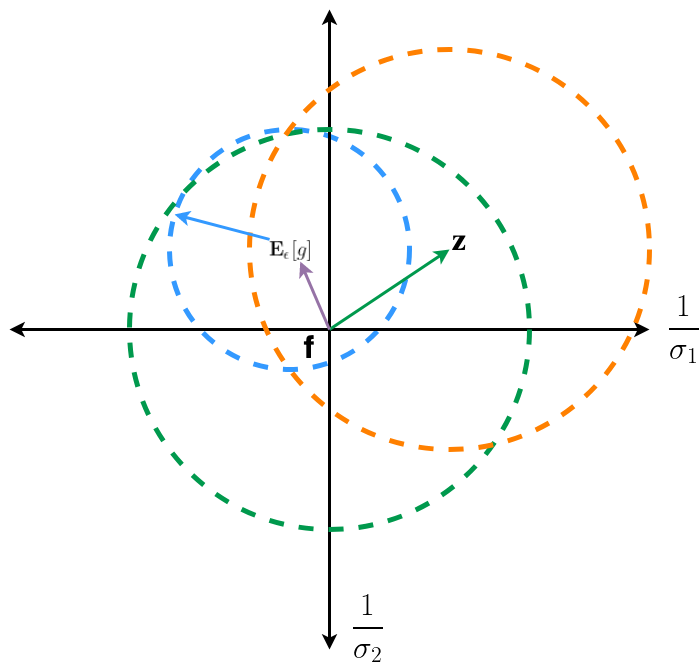
\includegraphics[width=0.8\textwidth]{diagonal_basis_2d_estimators_diagram.png}
    \caption{Example of geometric interpretation of closure test estimators. The origin
    is the predictions of the underlying law. The level one data is shifted away from this
    by $\shift$. In the basis which diagonalises the experimental covariance matrix, normalised by
    the square root of the eigenvalues, the 1-sigma noise vector confidence interval
    is a unit circle centered on the origin and the 1-sigma confidence interval
    of the level 2 data is a unit circle centered $\levone$. Some closure
    estimators can be understood as l2 norms of the vectors connecting points,
    i.e the bias is the l2 norm of the vector from the origin to the central
    value of the predictions.}
    \label{fig:diagram2destimators}
\end{figure}

In \eqref{eq:chi2decomp}, we implictly showed that $\Delta_{\chi^2}$ discussed
in the closure test of NNPDF3.0 is given by
\begin{equation}
    \Delta_{\chi^2} = {\rm bias} - {\rm cross\,term}.
\end{equation}
In the NNDPF3.0 paper, $\Delta_{\chi^2}$ was said to indicate under or overfitting
depending on its sign. Also it was said that $\Delta_{\chi^2}$ indicated that
the underlying law was reproduced. We can see with this decomposition that
if the underlying law is exactly obtained by the central value of the predictions,
$\Delta_{\chi^2}=0$, however $\Delta_{\chi^2}=0$ does not necessarily imply that
the underlying law is reproduced. On figure \ref{fig:diagram2destimators},
$\Delta_{\chi^2} = 0$ would define a hypersphere which is centered on the level
1 data and passes through the underlying law (so has radius equal to magnitude of
the vector from $\law$ to $\levone$). If $\Delta_{\chi^2} < 0$ then the central
value of the predictions lies within this hypersphere, similarly if
$\Delta_{\chi^2} > 0$ then the central value of the predictions lies outside
of this hypersphere. We should bear this in mind when talking about overfitting
with regards to both $\Delta_{\chi^2}$ and $\deltaeps$, we are specifically
defining that type of overfitting as fitting the fluctuated data better than
the underlying law. In the large $\ndata$ limit this manifests itself as
having enough freedom in the parameterisation that the minimum of the likelihood
function is lower than the expected value if the data were generated from that
model, this would be the case if $\chi^2 < 1$
(in a statistical significant way) or $\erep{\repchis} < 2$ for
$\Delta_{\chi^2}$ and $\erep{\Delta_{\repchis}}$ respectively. As previously discussed,
in the latter case there is an interplay between the overfitting of the central
predictions and the overfitting of the level two noise $\noise$ so it becomes
advantageous to consider $\Delta_{\chi^2}$ and $\deltaeps$ separately.

\subsection{Bias}

The {\em bias}\ is defined as the difference between the central value of the
replica predictions and the predictions obtained from the underlying law in
units of the covariance, \ie 
\begin{equation}
    \label{eq:BiasDef}
    \bias = \frac{1}{\ndata} \sum_{ij} \diffcentunder_i \invcov{ij} \diffcentunder_j.
\end{equation}
The smaller the bias, the closure the central value of the predictions is to
the underlying law. This is clearly a positive feature for a fit to have and so
we can use bias as a performance indicator, which can be used to distinguish
between two fitting methodologies which are used to fit the same closure test
data.

\subsection{Variance}

The {\em variance} in the above decomposition refers to the variance of the
replica predictions in units of the covariance
\begin{equation}
    \label{eq:VarDef}
    \var = \frac{1}{\ndata} \erep{ \sum_{ij} \diffcentrep_{i} \invcov{ij} \diffcentrep_{j}},
\end{equation}
which can be interpreted as the propagation of the PDF uncertainty in the space
of data. Specifically we can rewrite \eqref{eq:VarDef} as
\begin{equation}
    \label{eq:VarDefalternative}
    \var = \frac{1}{\ndata} {\rm Tr} \left[ \covrep \invcov{} \right],
\end{equation}
where $\covrep$ is the covariance matrix of the predictions
from the PDF replicas.
It is worth noting that both variance and bias can be determined
purely from the ensemble of PDF replicas and the underlying law.

It's clear that when choosing a fitting methodology we would like to minimise
both the bias and the variance: minimising the bias means that the central
value of the predictions is closer to the underlying law and minimising
the variance means that the PDF uncertainty is reduced. As dicussed in \cite{mlforphysics},
the general approach to reducing the bias is to
increase the number of parameters but this often has the side effect of
increasing the variance. In our case we have an additional subtlety, which is
the interplay between the bias and the variance.

\subsection{Multiple Closure Fits}

It should be fairly clear that the bias defined in \eqref{eq:BiasDef} will have
some dependence on the shift which is used to generate the level 1 data. We should
check whether or not the variance is as well. In a fit to experimental
data, we do not have any knowledge of the shift itself, rather the distribution
we assume that it is drawn from. Also, we can not generate a different shift
because the shift is fixed at the point that the experimental central values
are published.

In a closure test, however, we can in principle perform many
fits. Each fit can have independently generated level 1 data, as well as
level 2 replicas. Upon running many fits we can then take the expectation value
of the statistical estimators, bias and variance, across level 1 shifts. The expectation
of the bias across fits is given by
\begin{equation}
    \frac{1}{\ndata} \eshift{ \sum_{ij} \diffcentunder_i \invcov{ij} \diffcentunder_j },
\end{equation}
which, in analogy to \eqref{eq:VarDefalternative}, can be rewritten as
\begin{equation}
    \label{eq:BiasDefalternative}
    \bias = \frac{1}{\ndata} {\rm Tr} \left[ \covcent \invcov{} \right],
\end{equation}
except this time we have $\covcent$, the covariance of the central value
of predictions. If we consider the central value of the theory predictions for
a given fit as the reference point, then by rerunning multiple closure tests
we are effectively sampling from the probability distribution of the
difference between the central value of the predictions and the underlying law
predictions, $p(\diffcentunder)$. Earlier we mentioned that the aim of the NNPDF
methodology is for the PDF replicas about the central value of the predictions,
$q(\diffcentrep)$ to be representative of this distribution. The most common
method of determining how close these distributions are would be to calculate
the Kullback-Leibler (K-L) divergence between $p$ and $q$:
\begin{equation}
    D_{KL}(p || q) = \int_{-\infty}^{\infty} {\rm d} x \, p(x) \log \left(\frac{q(x)}{p(x)} \right).
\end{equation}
Note that the K-L divergence is not symmetric under the exchange of the reference
distribution, $p(x)$, in our case the observed distribution of the underlying law
about the central value of the prediction, and the model distribution, $q(x)$,
the model being the MC approach used in an NNPDF fit. If both the distributions,
$p(x)$ and $q(x)$ were multigaussian centered on the central value of the
predictions, with covariance $\covcent$ and
$\covrep$ respectively, then the K-L divergence simplifies to
% TODO: CHECK THIS!!!!!!!!
\begin{equation}
    D_{KL}(p || q) = \frac{1}{2} \left[
        \log\frac{|\covrep|}{|\covcent|}
        - \ndata
        + {\rm Tr} (\covcent {\covrep}^{-1})
        \right].
\end{equation}
% TODO: CHECK THIS!!!!!!!!
It is clear that if the covariance of the two distributions are equal, then
the K-L divergence goes to zero. It's also clear that if this is the case,
then we would expect that $\eshift{\bias}$ should be equal to $\var$. In reality,
getting a reasonable estimate of $\covcent$ and $\covrep$ would require a huge
number of fits, each with a large number of replicas. This would become
especially relevant when inverting the covariance matrix $\covrep$ in the case
that there were large correlations between theory predictions. In the next
section we will discuss estimators that require fewer statistics and attempt
to gauge the average behaviour of the two distributions across all data points.

The merit of running multiple closure tests is now becoming clear. On the one
hand we can check if one fitting methodology has a lower value of bias and
variance, averaged across fits. This gives us a performance indicator with
which we can rank fitting methodologies. In addition to this, we can validate
whether or not the PDF uncertainties, represented by the MC replicas for a given
fit, are "faithful". In NNPDF3.0 a first attempt to answer this was made,
at the time studies were limited by the length of
time it took to run a fit
and so instead of running multiple level 2 fits, single replicas fitted directly
to the level one data were used as proxies for full fits.

With the introduction of a faster fitting methodology it becomes feasible to
actually perform multiple level 2 closure fits with our proposed methodology,
and try to test how well the methodology performs, and whether uncertainties
are faithful.

\subsection{Bias Variance ratio}

If we were to perform multiple fits with different level-1
shifts and calculate the expectation value of the bias across fits,
$\eshift{\bias}$, then we can calculate
\begin{equation}
    \label{eq:BiasVarRatio}
    \frac{\eshift{\bias}}{\var} = 1.
\end{equation}
There is a clear geometric interpretation of this quantity.
In the basis which diagonalises the experimental
covariance matrix the variance is the mean squared radius of the replica predictions for a
given fit and the expected bias is the mean squared radius of the central value
of the predictions. We assume that the variance has a value which is
independent of $\shift$ and, with enough replicas, is constant across fits.
In practice we will also take the expectation value of $\var$ across fits,
because we will be running fits with finite replicas and so expect fluctuations
across fits.
% ALSO SHOULD CHECK IF VARIANCE DOES DEPEND ON LEVEL 1 SHIFT

We already saw that the form of $\eshift{\bias}$ is the same as $\var$ and that
the estimators are proportional to $\covcent$ and $\covrep$ respectively.
We could also have written variance in the basis which diagonalises the
experimental covariance matrix:
\begin{equation}
    \var = \frac{1}{\ndata} \erep{ \sum_{i} \frac{(\hat{\Delta}_{i, \noise})^2}{\hat{\sigma}_{i}^2}},
\end{equation}
where $\underline{\hat{\Delta}}$ is the vector of differences, $\diffcentrep$,
projected into the eigenbasis of the covmat and $\hat{\sigma}^2$ are the
eigenvalues of the covmat. If we take the expectation over replicas before
summing over the data points
\begin{equation}
    \var = \frac{1}{\ndata} \sum_{i} {\rm Var}(\frac{\hat{\Delta}_i}{\hat{\sigma}_i}),
\end{equation}
then we see that variance is the mean across data points of the second moment
of the distribution of replica predictions about the central value of the predictions.
A similar argument can be applied to $\eshift{\bias}$.

Then $\frac{\eshift{\bias}}{\eshift{\var}}$ is an estimate of whether the average
of the second moments of the distributions across data points is equal. Specifically
in units of the experimental covaraince matrix. It's clear that if the K-L
divergence between the distribution of the level 0 data about the
central prediction, $p(x)$, and the distribution of replica predictions about the central
prediction, $q(x)$, is zero then $\frac{\eshift{\bias}}{\eshift{\var}} = 1$
but that $\frac{\eshift{\bias}}{\eshift{\var}} = 1$ does not necessarily
imply that the K-L divergence is 0. Of course the ideal measurement would be
whether ${\rm Tr} (\covcent {\covrep}^{-1}) = \ndata$ but as discussed, despite
the improved performance of the fitting methodology, calulating this estimator
is still unfeasible but perhaps will be possible in a future iteration of the
NNPDF methodology.

It's perhaps not entirely obvious why we should consider the moments of the two
distributions in units of the experimental covariance. In the end this is a
practical choice, by doing this we are examining the differences in units which
the experimental data is most sensitive to, because directions which have lower
experimental uncertainty will contribute more to the bias and variance. This
seems like a good choice of units then, since in the end people will be comparing
theory predictions to experimental data, and so we prioritise having low bias
and low variance, as well as faithful uncertainties for directions in the space
of data for which we have low uncertainty.

\subsubsection{Quantile statistics}

A closure test estimator which was previously defined in PDF space was
$\xi_{1\sigma}$. We define here an analogous estimator in data space
\begin{equation}
    \label{eq:XiDataDef}
    \xi_{1\sigma} = 
        \frac{1}{\ndata} \sum_{i}^{\ndata} 
        \frac{1}{\nfits} \sum_{l}^{\nfits}
            I_{[-\sigma_i^{(l)}, \sigma_i^{(l)}]}
            \left( \erep{\model_i}^{(l)} - \law_i \right),
\end{equation}
where $\sigma^{(l)}$ is the standard deviation of the theory predictions
estimated from the replicas of fit $l$. $\xi_{1\sigma}$ aims to measure the same
thing as $\frac{\eshift{\bias}}{\eshift{\var}}$: whether the distribution of
replicas for a given fit matches the distribution of the central predictions
around the underlying predictions. It is useful to define $\xi_{1\sigma}^{i}$ as
the value of $\xi_{1\sigma}$ for an individual data point such that
\begin{equation}
    \label{eq:XiDataIDel}
    \xi_{1\sigma} = \frac{1}{\ndata} \sum_i \xi_{1\sigma}^{i}.
\end{equation}
If we assume that the replica distribution is constant across fits then our
definition $\xi_{1\sigma}^{i}$ is just a discretised expectation value of the
indicator function. In the case that we have infinite fits, then
\begin{equation}
    \label{eq:XiIExpecVel}
    \xi_{1\sigma}^{i} = 
    \int_{-\infty}^{\infty} I_{[-\sigma_i, \sigma_i]}\, 
    p(\erep{\model_i} - \law_i)\, 
    {\rm d}(\erep{\model_i} - \law_i).
\end{equation}
If we then assume that $p(\erep{\model_i} - \law_i)$ is a gaussian centered on
zero with a standard deviation which we will denote as $\modelstd_i$ then the
integral simplifies to
\begin{equation}
    \label{eq:expectedxi}
    \xi_{1\sigma}^{i} = 
    \erf \left( \frac{\sigma_i}{\modelstd_i \sqrt{2}}\right),
\end{equation}
which is the standard result of integrating a gaussian over some finite
symmetric interval. Clearly if the distribution of central predictions about the
underlying law matches the distribution of the replica predicitons around the
central predictions then the expected value of $\xi_{1\sigma}^{i}$ is 0.68. This
is consistent with the assumptions we made, \viz\ it is  the quantile statistics
of a gaussian distribution.

One can also look at the variance of the indicator function across fits to get
an idea of the fluctuation of $\xi_{1\sigma}^{i}$, which we will denote as
$\Delta[\xi_{1\sigma}^{i}]$
\begin{equation}
    \label{eq:XiIVar}
    \begin{split}
        \Delta[\xi_{1\sigma}^{i}] 
        =& \int_{-\infty}^{\infty} I_{[-\sigma_i, \sigma_i]}^2\, 
            p(\erep{\model_i} - \law_i)\,
            {\rm d}(\erep{\model_i} - \law_i) - \\
        &- \left( \int_{-\infty}^{\infty} I_{[-\sigma_i, \sigma_i]}\,
            p(\erep{\model_i} - \law_i)\,
            {\rm d}(\erep{\model_i} - \law_i) \right)^2,
    \end{split}
\end{equation}
which can be simplified to
\begin{equation}
    \label{eq:XiIVarSimplified}
    \Delta[\xi_{1\sigma}^{i}] =
    \erf \left( \frac{\sigma_i}{\modelstd_i \sqrt{2}}\right) -
    \erf \left( \frac{\sigma_i}{\modelstd_i \sqrt{2}}\right)^2.
\end{equation}
Even in the ideal case that the distributions are the same, we see that the
$\Delta[\xi_{1\sigma}^{i}] = 0.22$, which is a large spread considering
$\xi_{1\sigma}^{i}$ is bounded between 0 and 1.

When taking the mean across datapoints to obtain $\xi_{1\sigma}$ we note that
getting 0.68 relies on each sampled $\xi_{1\sigma}^{i}$ being statistically
independent. This clearly will not be the case because there can be a big
correlation between datapoints within the same dataset. We can calculate
$\xi_{1\sigma}$ in different basis and note that unlike $\chi^2$ and quantities
of the form $v^T M v$, $\xi_{1\sigma}$ is not basis independent. There is a
choice of basis, however it will be useful to compare the value $\xi_{1\sigma}$
and $\frac{\eshift{\bias}}{\eshift{\var}}$. Therefore, a natural basis to
calculate $\xi_{1\sigma}$ is the basis which diagonalises the experimental
covariance matrix because bias and variance are both calculated in units of the
experimental
% Should I mention this without having tried it?
covariance. As previously discussed, this makes sense in light of using the PDFs
to make data-theory comparisons.

\subsection{Out of sample}

We want to calculate the closure test estimators on data which is out of sample
to check uncertainty is faithful on new predictions and that the bias and variance
are lower for out of sample data. We can choose to calculate \eqref{eq:chi2kerep}
on data which is not used in the fit, in which case we refer to $\erep{\repchis}$
the expected generalisation error. This is relevant because in general people
will be using our PDFs to make predictions on data which has not been fitted
and so it is particularly important that the performance is good, and that the
PDF uncertainties are faithful when the data hasn't been fitted.

In order to do this, we should determine the requirements for out of sample data.
Here we should discuss the theory prediction correlations as well as the
decomposition only making sense if the experimental data is uncorrelated between
in sample and out of sample.
